\documentclass[nofonts]{tufte-handout}

\usepackage{polyglossia}
\setdefaultlanguage{french}
\usepackage{booktabs}
\usepackage[locale=FR]{siunitx}
\usepackage{graphicx}
\usepackage{enumitem}
\usepackage{tikz}
\usepackage{amsmath}

\usepackage{fontspec}
\usepackage{ifluatex}
\setmainfont[Renderer=Basic, Numbers=OldStyle, Scale = 1.0]{TeX Gyre Pagella}
\setsansfont[Renderer=Basic, Scale=0.90]{TeX Gyre Heros}
\setmonofont[Renderer=Basic]{TeX Gyre Cursor}
\ifluatex
  \newcommand{\textls}[2][5]{%
    \begingroup\addfontfeatures{LetterSpace=#1}#2\endgroup
  }
  \renewcommand{\allcapsspacing}[1]{\textls[15]{#1}}
  \renewcommand{\smallcapsspacing}[1]{\textls[10]{#1}}
  \renewcommand{\allcaps}[1]{\textls[15]{\MakeTextUppercase{#1}}}
  \renewcommand{\smallcaps}[1]{\smallcapsspacing{\scshape\MakeTextLowercase{#1}}}
  \renewcommand{\textsc}[1]{\smallcapsspacing{\textsmallcaps{#1}}}
\fi

\sisetup{
  mode=text,
  reset-text-family=false,
  reset-text-series=false,
  per-mode=symbol,
}

\newcommand{\F}{\boldsymbol{F}}
\newcommand{\vv}{\boldsymbol{v}}

\title{Exercices de révision de mécanique}
\author{Loïc Séguin-Charbonneau}
\date{203-NYB-05, Automne 2024}

\begin{document}

\maketitle

\section{Lancer du marteau}

Aux Jeux olympiques de Paris, la Canadienne Camryn Rogers a lancé le marteau à
une distance de \qty{76.97}{\meter} ce qui lui a valu la médaille d'or. L'angle
que faisait la vitesse du marteau avec l'horizontal au moment du lancer était
de \qty{39.02}{\degree}. À ce moment, le boulet était environ à la
hauteur de la tête de l'athlète, soit \qty{170}{\centi\meter}. La longueur du marteau est
de \qty{1195}{\milli\meter} et sa masse de \qty{4}{\kilo\gram}.
\begin{marginfigure}
  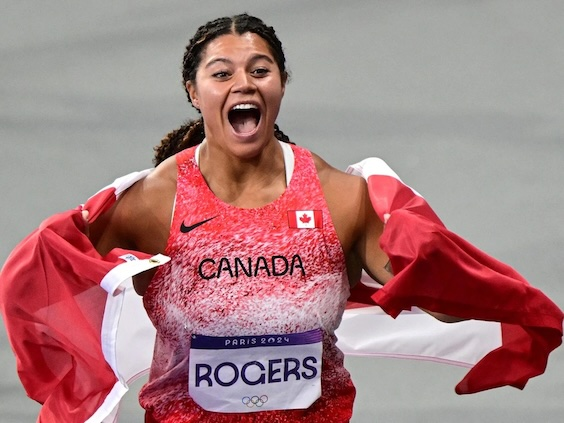
\includegraphics[width=\marginparwidth]{figures/camryn_rogers.jpg}
  \caption{Camryn Rogers après avoir gagné la médaille d'or aux Jeux olympiques
  de Paris. Photo par Martin Bernetti/AFP}
\end{marginfigure}

\begin{enumerate}[label=\alph*)]
  \item Quelle était la vitesse du marteau au moment de le lâcher?
  \item Quelle était la hauteur maximale atteinte par le marteau?
  \item Juste avant de lâcher le marteau, quelle force devait exercer Camryn
    pour le maintenir en rotation?
\end{enumerate}



\section{Énergie et puissance d'un barrage hydroélectrique}

La centrale hydroélectrique Robert-Bourassa sur la rivière La Grande est une
centrale à réservoir. L'eau du réservoir chute d'une hauteur de
\qty{137.16}{\meter} et fait tourner une turbine reliée à une génératrice. La
centrale produit une puissance électrique de \qty{5616}{\mega\watt}.

\begin{enumerate}[label=\alph*)]
  \item Quelle est l'énergie potentielle d'un kilogramme d'eau au sommet du réservoir?
  \item Quelle est l'énergie cinétique d'un kilogramme d'eau juste avant qu'il
    ne touche la turbine en bas du réservoir?
  \item La centrale a une efficacité de \qty{90}{\percent}, c'est-à-dire que
    \qty{90}{\percent} de l'énergie cinétique de l'eau qui tombe peut être
    convertie en énergie électrique. Quelle quantité d'énergie électrique est
    produit par la chute d'un kilogramme d'eau?
  \item Quelle masse d'eau est requise pour produire \qty{5616}{\mega\joule} d'énergie?
  \item Quel débit d'eau (c'est-à-dire le volume par unité de temps) doit
    tomber pour produire une puissance de \qty{5616}{\mega\watt}?
\end{enumerate}

\newpage

\section{Forces sur un vaisseau spatial}

Un satellite de \qty{156}{\kilogram} est en orbite autour de la Terre à une
altitude de \qty{400}{\kilo\meter}. Le satellite allume un propulseur qui
éjecte un gaz générant une force $\F_p$ de \qty{170}{\newton} qui
fait un angle de \SI{125}{\degree} avec la vitesse du vaisseau (voir la figure
ci-contre).
\begin{marginfigure}
  \begin{tikzpicture}[>=stealth]
    \draw (0, 0) circle (2cm);
    \fill[black!70] (0, 0) circle (12px);
    \begin{scope}[shift={(0.3, 2.2cm)}, scale=0.3, rotate=150]
      \draw[fill=black!60] (0, 0) rectangle (1, 2);
      \draw (0.5, 2) -- ++(80:0.9);
      \draw (0.5, 2) -- ++(100:1.1);
      \draw (1, 1) -- ++(10:1) rectangle ++(0.4, 0.6);
      \draw (0, 1) -- ++(190:1) rectangle ++(-0.4, +0.6);
    \end{scope}
    \draw[ultra thick, ->] (0, 2) -- ++(1, 0) node[above] {$\vv$};
    \draw[ultra thick, ->] (0, 2) -- ++(125: 1.3) node[above] {$\F_p$};
    \draw (0.5, 2) arc (0: 125: 0.5);
    \node at (0.4, 2.6) {\qty{125}{\degree}};
  \end{tikzpicture}
\end{marginfigure}

\begin{enumerate}[label=\alph*)]
  \item Quelle est la force nette qui agit sur le satellite?
  \item La force agit pendant quelques secondes, puis le propulseur est éteint.
    En supposant que le satellite continue de faire un mouvement circulaire
    autour de la Terre, sont altitude sera-t-elle plus grande ou plus petite
    qu'avant l'allumage du propulseur?
\end{enumerate}


\section{Un vol d'une seconde}
\marginnote{Chapitre 1, exercice 1.10.5 dans \citet{seguin_mec_2024}}
À quel angle doit-on lancer une balle à \qty{8}{\meter\per\second} pour qu'elle
reste dans les airs pendant \qty{1}{\second}?


\section{Volleyball}
\marginnote{Chapitre 4, P27 dans \citet{lafrance_mec_2014}}
Au volleyball, le filet a une hauteur de \qty{2.43}{\meter} et il est situé à
une distance de \qty{9}{\meter} du serveur. Ce dernier frappe le ballon à une
vitesse de \qty{12.4}{\meter\per\second}, formant un angle de
\qty{24.0}{\degree} au-dessus de l'horizontale et à une hauteur de
\qty{2.2}{\meter}.
\begin{enumerate}[label=\alph*)]
  \item À quelle hauteur au-dessus du filet le ballon passe-t-il?
  \item Donnez le module et l'orientation de la vitesse à ce moment.
  \item À quelle distance du filet le ballon frappe-t-il le sol?
\end{enumerate}


\section{Plan incliné}
\marginnote{Chapitre 6, E21 dans \citet{benson_mec_2024}}
Deux blocs de masses égales $m_1 = m_2 = \qty{5}{\kilo\gram}$ sont reliés entre
eux et suspendus à une poulie. On donne $\mu_c = \num{0.25}$ pour le bloc 2.
Trouver le module de l'accélération des deux blocs sachant que $m_1$ se déplace
vers le bas.
\begin{marginfigure}
  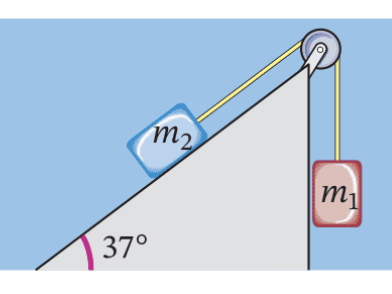
\includegraphics[width=\marginparwidth]{figures/benson_c6e21.png}
\end{marginfigure}


\section{Réponses}

\noindent Un vol d'une seconde : \qty{37.8}{\degree} au-dessus de l'horizontal

\noindent Volleyball: a) \qty{0.68}{\meter};
            b) \qty{11.7}{\meter\per\second} à \qty{13.6}{\degree} sous l'horizontale;
            c) \qty{6.4}{\meter}

\noindent Plan incliné: \qty{0.980}{\meter\per\second\squared}

\bibliography{../elecmag}
\bibliographystyle{plainnat}

\end{document}

